%%%%%%%%%%%%%%%%%%%%%%%%%%%%%%%%%%%%%%%%%
% Beamer Presentation
% LaTeX Template
% Version 1.0 (10/11/12)
%
% This template has been downloaded from:
% http://www.LaTeXTemplates.com
%
% License:
% CC BY-NC-SA 3.0 (http://creativecommons.org/licenses/by-nc-sa/3.0/)
%
%%%%%%%%%%%%%%%%%%%%%%%%%%%%%%%%%%%%%%%%%

%----------------------------------------------------------------------------------------
%	PACKAGES AND THEMES
%----------------------------------------------------------------------------------------

\documentclass{beamer}
\usepackage{fontspec}
\usepackage{bibentry}
\setmainfont{Times-Roman}
\setsansfont{SourceSerifPro-Regular}
\setmonofont{CascadiaCode}
\setbeamertemplate{frametitle}[default][center]

\mode<presentation> {

% The Beamer class comes with a number of default slide themes
% which change the colors and layouts of slides. Below this is a list
% of all the themes, uncomment each in turn to see what they look like.

\usetheme{default}
%\usetheme{AnnArbor}
%\usetheme{Antibes}
%\usetheme{Bergen}
%\usetheme{Berkeley}
%\usetheme{Berlin}
%\usetheme{Boadilla}
%\usetheme{CambridgeUS}
%\usetheme{Copenhagen}
%\usetheme{Darmstadt}
%\usetheme{Dresden}
%\usetheme{Frankfurt}
%\usetheme{Goettingen}
%\usetheme{Hannover}
%\usetheme{Ilmenau}
%\usetheme{JuanLesPins}
%\usetheme{Luebeck}
%\usetheme{Madrid}
%\usetheme{Malmoe}
%\usetheme{Marburg}
%\usetheme{Montpellier}
%\usetheme{PaloAlto}
%\usetheme{Pittsburgh}
%\usetheme{Rochester}
%\usetheme{Singapore}
%\usetheme{Szeged}
%\usetheme{Warsaw}

% As well as themes, the Beamer class has a number of color themes
% for any slide theme. Uncomment each of these in turn to see how it
% changes the colors of your current slide theme.

%\usecolortheme{albatross}
%\usecolortheme{beaver}
%\usecolortheme{beetle}
%\usecolortheme{crane}
%\usecolortheme{dolphin}
%\usecolortheme{dove}
%\usecolortheme{fly}
%\usecolortheme{lily}
%\usecolortheme{orchid}
%\usecolortheme{rose}
%\usecolortheme{seagull}
%\usecolortheme{seahorse}
%\usecolortheme{whale}
%\usecolortheme{wolverine}

%\setbeamertemplate{footline} % To remove the footer line in all slides uncomment this line
%\setbeamertemplate{footline}[page number] % To replace the footer line in all slides with a simple slide count uncomment this line

%\setbeamertemplate{navigation symbols}{} % To remove the navigation symbols from the bottom of all slides uncomment this line
}

\usepackage{graphicx} % Allows including images
\usepackage{booktabs} % Allows the use of \toprule, \midrule and \bottomrule in tables

%----------------------------------------------------------------------------------------
%	TITLE PAGE
%----------------------------------------------------------------------------------------

\title[GAI based on ML]{Recommendation Ranking based on online comment mining and sentiment analysis} % The short title appears at the bottom of every slide, the full title is only on the title page

\author{ Wangzhihui Mei, Hongyi Huang, Liting Lv, Yueyue He} % Your name
\institute[JI] % Your institution as it will appear on the bottom of every slide, may be shorthand to save space
{
CCNU-UOW JI \\ % Your institution for the title page
\medskip
\textit{maywzh@gmail.com} % Your email address
}
\date{\today} % Date, can be changed to a custom date

\begin{document}

\begin{frame}
    \titlepage % Print the title page as the first slide
\end{frame}

\begin{frame}
    \frametitle{Overview} % Table of contents slide, comment this block out to remove it
    \tableofcontents % Throughout your presentation, if you choose to use \section{} and \subsection{} commands, these will automatically be printed on this slide as an overview of your presentation
\end{frame}

%----------------------------------------------------------------------------------------
%	PRESENTATION SLIDES
%----------------------------------------------------------------------------------------

%------------------------------------------------
\section{Introduction} % Sections can be created in order to organize your presentation into discrete blocks, all sections and subsections are automatically printed in the table of contents as an overview of the talk
%------------------------------------------------

\begin{frame}
    \frametitle{Introduction}
    The Recommendation Ranking is the process of generating business content for users depend on user's interests and hobbies. We are introducting an approach that using online comment mining and sentiment analysis to for its implementation.
\end{frame}

\begin{frame}
    \frametitle{Background}
    With the rapid increase in online review content, the consumer experience of users has become tangible. The development of sentiment analysis technology and text mining technology has greatly enhanced the ability of merchants to perceive customer needs and provide timely feedback.
\end{frame}

\section{Problems}
\begin{frame}
    \frametitle{Problems}
    \begin{itemize}
        \item which reviews are useful?
        \item how can we combine useful online reviews with classic research models?
    \end{itemize}
\end{frame}

\section{Methodology}
\begin{frame}
    \frametitle{Methodology}
    \begin{itemize}
        \item Data pre-procession
        \item Data Helpfulness analysis
        \item Sentiment Analysis
    \end{itemize}
\end{frame}

\subsection{Data pre-procession}
\begin{frame}
    \frametitle{Data pre-procession}
    A large number of online reviews are text, and text is unstructured content. If modeling is needed, it needs to be converted into structured, analyzable, and quantifiable content. Regarding data collection and preprocessing, we first conduct research, crawling, thesaurus construction, and sentiment analysis, and then transform it into structured data and input it into the second and third modules.
    \begin{figure}[]
        \centering
        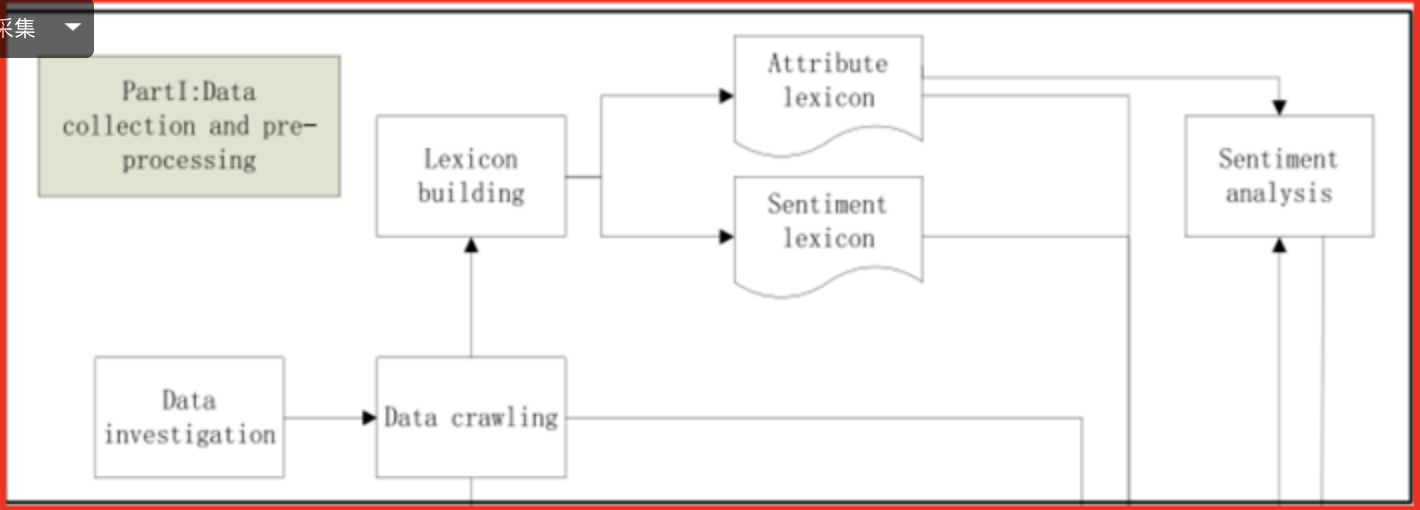
\includegraphics[width=0.6\linewidth]{fig/preprocess}
        \caption{Preprocess}
    \end{figure}
\end{frame}

\subsection{Data Helpfulness analysis}
\begin{frame}
    \frametitle{Data Helpfulness analysis}
    The unevenness of the quality of reviews seriously interferes with the accuracy and credibility of demand mining. How to find useful comments that can accurately describe user needs is a prerequisite guarantee for improving the effectiveness of demand acquisition technology. Aiming at this problem, this article proposes a method for analyzing the usefulness of reviews based on complex networks, using the semantic relationship between reviews to analyze the reviews from a macro perspective.
    \begin{figure}[]
        \centering
        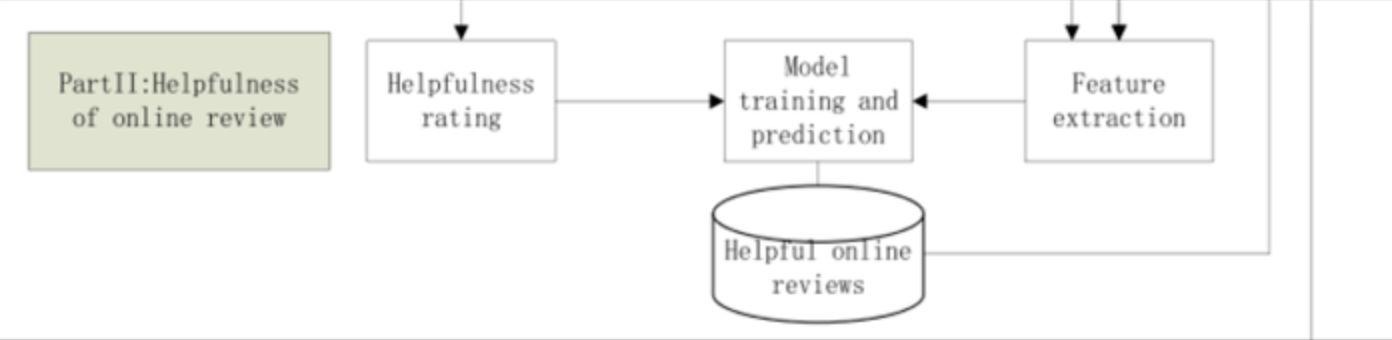
\includegraphics[width=0.6\linewidth]{fig/help}
        \caption{Data Helpfulness Process}
    \end{figure}

\end{frame}
%------------------------------------------------

\subsection{Sentiment Analysis}
\begin{frame}
    \frametitle{Sentiment Analysis}
    How to mine evaluation objects that have appeared in the text. There are four main methods, namely noun mining, association of evaluation words and objects, supervised learning methods, and topic models.
    \begin{figure}[]
        \centering
        
\includegraphics[width=0.6\linewidth]{fig/sean}
        \caption{5 Factors of Sentiment Analysis}
    \end{figure}
\end{frame}

\section{Reference}
\begin{frame}[allowframebreaks]
    \frametitle{Reference}
    \begin{figure}[]
        \centering
        
\includegraphics[width=0.6\linewidth]{fig/ref1}

    \end{figure}
    \begin{figure}[]
        \centering
        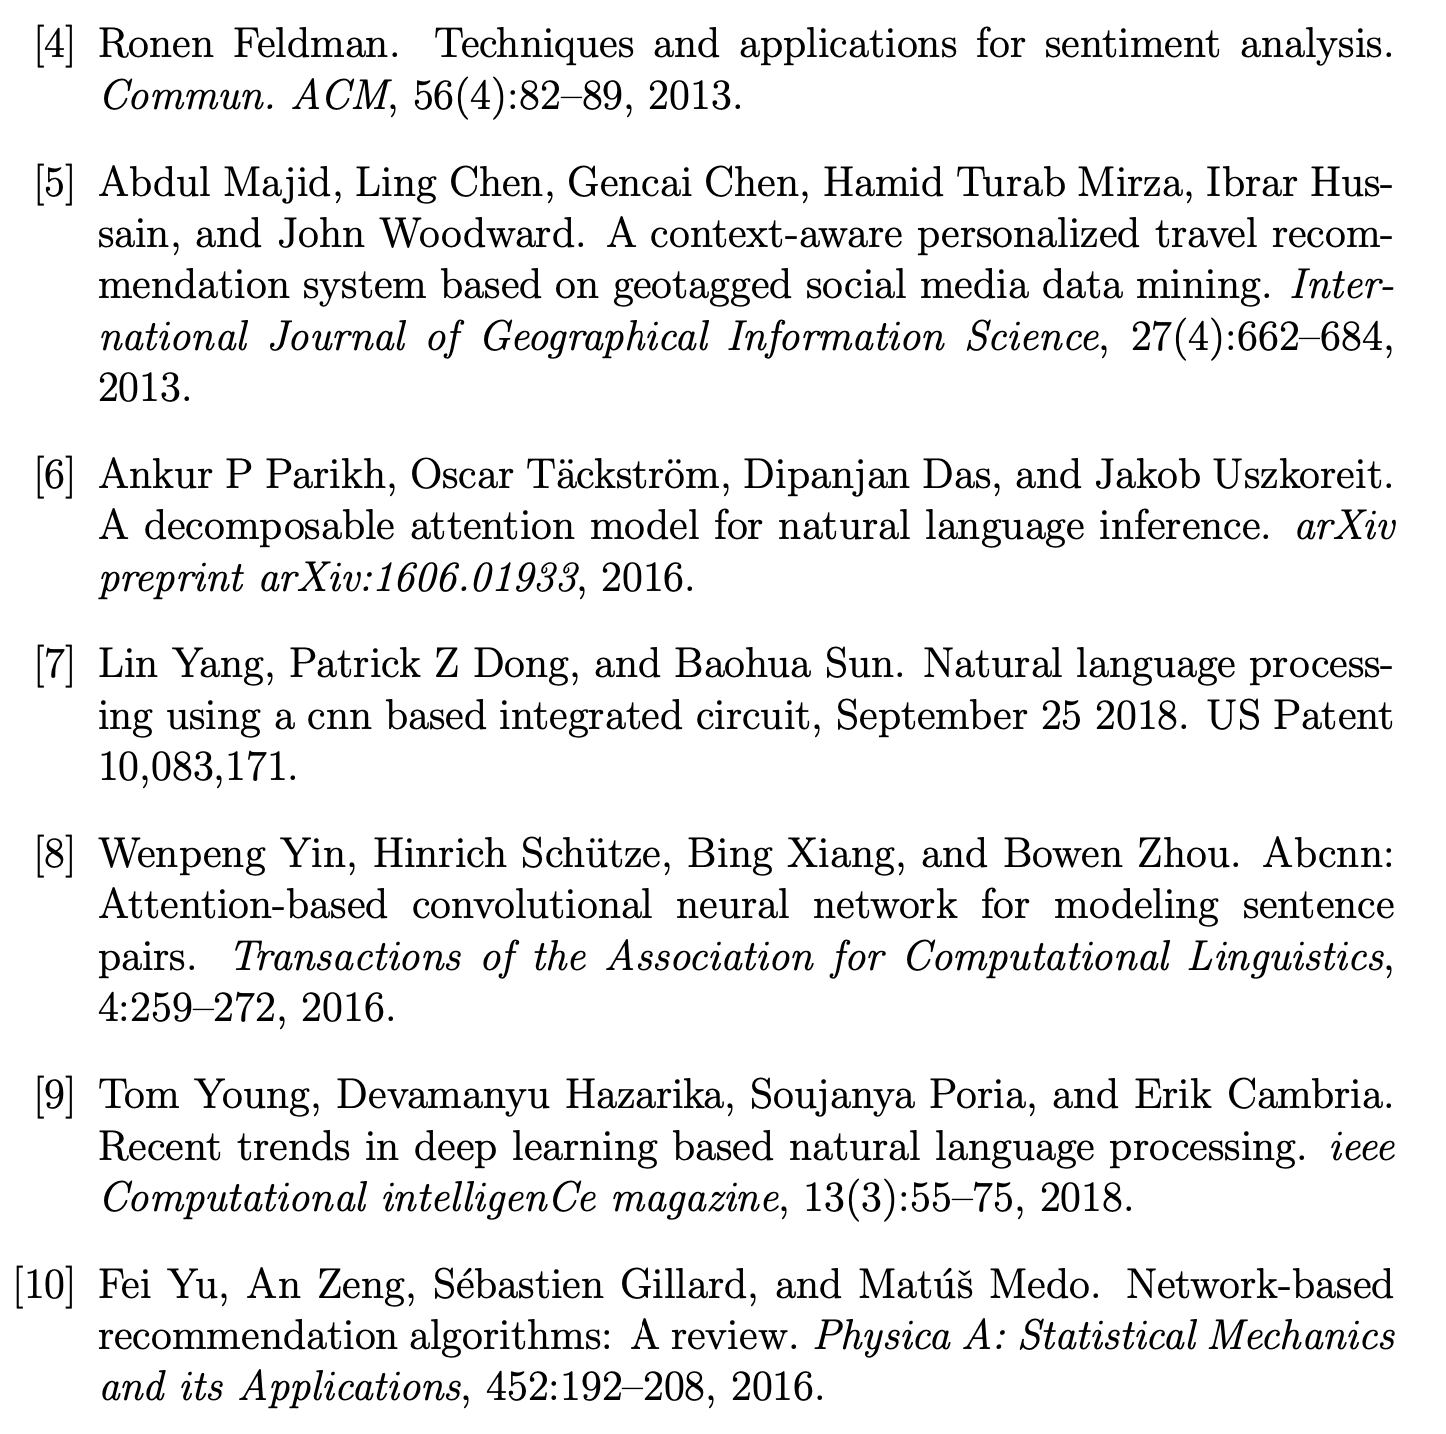
\includegraphics[width=0.6\linewidth]{fig/ref2}

    \end{figure}

\end{frame}
\begin{frame}
    \Huge{\centerline{The End}}
\end{frame}

%----------------------------------------------------------------------------------------

\end{document}